\documentclass{article}

%%%% packages and definitions (optional)
\usepackage{graphicx} % allows inclusion of graphics
\usepackage{graphics}
\usepackage{placeins}
\usepackage{booktabs} % nice rules (thick lines) for tables
\usepackage{microtype} % improves typography for PDF
\usepackage{xspace}
\usepackage[hidelinks]{hyperref}
\usepackage{xspace}
\usepackage{hhline}

\usepackage{tabularx}
\newcolumntype{b}{X}
\newcolumntype{s}{>{\hsize=.5\hsize}X}
\newcolumntype{m}{>{\hsize=.75\hsize}X}

\newcommand{\SN}{S$_N$}
\renewcommand{\vec}[1]{\bm{#1}} %vector is bold italic
\newcommand{\vd}{\bm{\cdot}} % slightly bold vector dot
\newcommand{\grad}{\vec{\nabla}} % gradient
\newcommand{\ud}{\mathop{}\!\mathrm{d}} % upright derivative symbol
\newcommand{\Cyclus}{\textsc{Cyclus}\xspace}%
\graphicspath{ {images/} }
\usepackage[affil-it]{authblk}
\usepackage{tikz}
\usetikzlibrary{positioning, arrows, decorations, shapes }
\usepackage{cleveref}

\usepackage{datatool}
\usepackage[acronym,toc]{glossaries}
%\newacronym{<++>}{<++>}{<++>}
\newacronym[longplural={metric tons of heavy metal}]{MTHM}{MTHM}{metric ton of heavy metal}
\newacronym{ABM}{ABM}{agent-based modeling}
\newacronym{ACDIS}{ACDIS}{Program in Arms Control \& Domestic and International Security}
\newacronym{ADS}{ADS}{Accelerator-Driven System}
\newacronym{AHTR}{AHTR}{Advanced High Temperature Reactor}
\newacronym{ANDRA}{ANDRA}{Agence Nationale pour la gestion des D\'echets RAdioactifs, the French National Agency for Radioactive Waste Management}
\newacronym{ANL}{ANL}{Argonne National Laboratory}
\newacronym{ANS}{ANS}{American Nuclear Society}
\newacronym{API}{API}{application programming interface}
\newacronym{ARE}{ARE}{Aircraft Reactor Experiment}
\newacronym{ARFC}{ARFC}{Advanced Reactors and Fuel Cycles}
\newacronym{ASME}{ASME}{American Society of Mechanical Engineers}
\newacronym{ASTRID}{ASTRID}{Advanced Sodium Technological Reactor for Industrial Demonstration}
\newacronym{ATWS}{ATWS}{Anticipated Transient Without Scram}
\newacronym{BDBE}{BDBE}{Beyond Design Basis Event}
\newacronym{BIDS}{BIDS}{Berkeley Institute for Data Science}
\newacronym{BWR}{BWR}{Boiling Water Reactor}
\newacronym{CAFCA}{CAFCA}{ Code for Advanced Fuel Cycles Assessment }
\newacronym{CDTN}{CDTN}{Centro de Desenvolvimento da Tecnologia Nuclear}
\newacronym{CEA}{CEA}{Commissariat \`a l'\'Energie Atomique et aux \'Energies Alternatives}
\newacronym{CI}{CI}{continuous integration}
\newacronym{CNEN}{CNEN}{Comiss\~{a}o Nacional de Energia Nuclear}
\newacronym{CNERG}{CNERG}{Computational Nuclear Engineering Research Group}
\newacronym{COSI}{COSI}{Commelini-Sicard}
\newacronym{COTS}{COTS}{commercial, off-the-shelf}
\newacronym{CSNF}{CSNF}{commercial spent nuclear fuel}
\newacronym{CTAH}{CTAHs}{Coiled Tube Air Heaters}
\newacronym{CUBIT}{CUBIT}{CUBIT Geometry and Mesh Generation Toolkit}
\newacronym{CURIE}{CURIE}{Centralized Used Fuel Resource for Information Exchange}
\newacronym{DAG}{DAG}{directed acyclic graph}
\newacronym{DANESS}{DANESS}{Dynamic Analysis of Nuclear Energy System Strategies}
\newacronym{DBE}{DBE}{Design Basis Event}
\newacronym{DESAE}{DESAE}{Dynamic Analysis of Nuclear Energy Systems Strategies}
\newacronym{DHS}{DHS}{Department of Homeland Security}
\newacronym{DOE}{DOE}{Department of Energy}
\newacronym{DRACS}{DRACS}{Direct Reactor Auxiliary Cooling System}
\newacronym{DRE}{DRE}{dynamic resource exchange}
\newacronym{DSNF}{DSNF}{DOE spent nuclear fuel}
\newacronym{DYMOND}{DYMOND}{Dynamic Model of Nuclear Development }
\newacronym{EBS}{EBS}{Engineered Barrier System}
\newacronym{EDF}{EDF}{Électricité de France}
\newacronym{EDZ}{EDZ}{Excavation Disturbed Zone}
\newacronym{EIA}{EIA}{U.S. Energy Information Administration}
\newacronym{EPA}{EPA}{Environmental Protection Agency}
\newacronym{EPR}{EPR}{European Pressurized Reactor}
\newacronym{EP}{EP}{Engineering Physics}
\newacronym{EU}{EU}{European Union}
\newacronym{FCO}{FCO}{Fuel Cycle Options}
\newacronym{FCT}{FCT}{Fuel Cycle Technology}
\newacronym{FEHM}{FEHM}{Finite Element Heat and Mass Transfer}
\newacronym{FEPs}{FEPs}{Features, Events, and Processes}
\newacronym{FHR}{FHR}{Fluoride-Salt-Cooled High-Temperature Reactor}
\newacronym{FLiBe}{FLiBe}{Fluoride-Lithium-Beryllium}
\newacronym{FP}{FP}{Fission Products}
\newacronym{GDSE}{GDSE}{Generic Disposal System Environment}
\newacronym{GDSM}{GDSM}{Generic Disposal System Model}
\newacronym{GENIUSv1}{GENIUSv1}{Global Evaluation of Nuclear Infrastructure Utilization Scenarios, Version 1}
\newacronym{GENIUSv2}{GENIUSv2}{Global Evaluation of Nuclear Infrastructure Utilization Scenarios, Version 2}
\newacronym{GENIUS}{GENIUS}{Global Evaluation of Nuclear Infrastructure Utilization Scenarios}
\newacronym{GPAM}{GPAM}{Generic Performance Assessment Model}
\newacronym{GRSAC}{GRSAC}{Graphite Reactor Severe Accident Code}
\newacronym{GUI}{GUI}{graphical user interface}
\newacronym{GWe}{GWe}{gigawatts electric}
\newacronym{HLW}{HLW}{high level waste}
\newacronym{HPC}{HPC}{high-performance computing}
\newacronym{HTC}{HTC}{high-throughput computing}
\newacronym{HTGR}{HTGR}{High Temperature Gas-Cooled Reactor}
\newacronym{IAEA}{IAEA}{International Atomic Energy Agency}
\newacronym{IEMA}{IEMA}{Illinois Emergency Mangament Agency}
\newacronym{IHLRWM}{IHLRWM}{International High Level Radioactive Waste Management}
\newacronym{INL}{INL}{Idaho National Laboratory}
\newacronym{IPRR1}{IRP-R1}{Instituto de Pesquisas Radioativas Reator 1}
\newacronym{IRP}{IRP}{Integrated Research Project}
\newacronym{ISFSI}{ISFSI}{Independent Spent Fuel Storage Installation}
\newacronym{ISRG}{ISRG}{Independent Student Research Group}
\newacronym{JFNK}{JFNK}{Jacobian-Free Newton Krylov}
\newacronym{LANL}{LANL}{Los Alamos National Laboratory}
\newacronym{LBNL}{LBNL}{Lawrence Berkeley National Laboratory}
\newacronym{LCOE}{LCOE}{levelized cost of electricity}
\newacronym{LDRD}{LDRD}{laboratory directed research and development}
\newacronym{LFR}{LFR}{Lead-Cooled Fast Reactor}
\newacronym{LLNL}{LLNL}{Lawrence Livermore National Laboratory}
\newacronym{LMFBR}{LMFBR}{Liquid Metal Fast Breeder Reactor}
\newacronym{LOFC}{LOFC}{Loss of Forced Cooling}
\newacronym{LOHS}{LOHS}{Loss of Heat Sink}
\newacronym{LOLA}{LOLA}{Loss of Large Area}
\newacronym{LP}{LP}{linear program}
\newacronym{LWR}{LWR}{Light Water Reactor}
\newacronym{MAGNOX}{MAGNOX}{Magnesium Alloy Graphie Moderated Gas Cooled Uranium Oxide Reactor}
\newacronym{MA}{MA}{minor actinide}
\newacronym{MCNP}{MCNP}{Monte Carlo N-Particle code}
\newacronym{MILP}{MILP}{mixed-integer linear program}
\newacronym{MIT}{MIT}{the Massachusetts Institute of Technology}
\newacronym{MOAB}{MOAB}{Mesh-Oriented datABase}
\newacronym{MOOSE}{MOOSE}{Multiphysics Object-Oriented Simulation Environment}
\newacronym{MOX}{MOX}{Mixed Oxide Fuel}
\newacronym{MSBR}{MSBR}{Molten Salt Breeder Reactor}
\newacronym{MSRE}{MSRE}{Molten Salt Reactor Experiment}
\newacronym{MSR}{MSR}{Molten Salt Reactor}
\newacronym{MWe}{MWe}{megawatts electric}
\newacronym{NAGRA}{NAGRA}{National Cooperative for the Disposal of Radioactive Waste}
\newacronym{NEAMS}{NEAMS}{Nuclear Engineering Advanced Modeling and Simulation}
\newacronym{NEUP}{NEUP}{Nuclear Energy University Programs}
\newacronym{NFCSim}{NFCSim}{Nuclear Fuel Cycle Simulator}
\newacronym{NGNP}{NGNP}{Next Generation Nuclear Plant}
\newacronym{NMWPC}{NMWPC}{Nuclear MW Per Capita}
\newacronym{NNSA}{NNSA}{National Nuclear Security Administration}
\newacronym{NPRE}{NPRE}{Department of Nuclear, Plasma, and Radiological Engineering}
\newacronym{NQA1}{NQA-1}{Nuclear Quality Assurance - 1}
\newacronym{NRC}{NRC}{Nuclear Regulatory Commission}
\newacronym{NSF}{NSF}{National Science Foundation}
\newacronym{NSSC}{NSSC}{Nuclear Science and Security Consortium}
\newacronym{NUWASTE}{NUWASTE}{Nuclear Waste Assessment System for Technical Evaluation}
\newacronym{NWF}{NWF}{Nuclear Waste Fund}
\newacronym{NWTRB}{NWTRB}{Nuclear Waste Technical Review Board}
\newacronym{OCRWM}{OCRWM}{Office of Civilian Radioactive Waste Management}
\newacronym{ORION}{ORION}{ORION}
\newacronym{ORNL}{ORNL}{Oak Ridge National Laboratory}
\newacronym{PARCS}{PARCS}{Purdue Advanced Reactor Core Simulator}
\newacronym{PBAHTR}{PB-AHTR}{Pebble Bed Advanced High Temperature Reactor}
\newacronym{PBFHR}{PB-FHR}{Pebble-Bed Fluoride-Salt-Cooled High-Temperature Reactor}
\newacronym{PEI}{PEI}{Peak Environmental Impact}
\newacronym{PHWR}{Pressurized Heavy Water Reactor}{Pressurized Heavy Water Reactor}
\newacronym{PH}{PRONGHORN}{PRONGHORN}
\newacronym{PRIS}{PRIS}{Power Reactor Information System}
\newacronym{PRKE}{PRKE}{Point Reactor Kinetics Equations}
\newacronym{PSPG}{PSPG}{Pressure-Stabilizing/Petrov-Galerkin}
\newacronym{PWAR}{PWAR}{Pratt and Whitney Aircraft Reactor}
\newacronym{PWR}{PWR}{Pressurized Water Reactor}
\newacronym{PyNE}{PyNE}{Python toolkit for Nuclear Engineering}
\newacronym{PyRK}{PyRK}{Python for Reactor Kinetics}
\newacronym{QA}{QA}{quality assurance}
\newacronym{RDD}{RD\&D}{Research Development and Demonstration}
\newacronym{RD}{R\&D}{Research and Development}
\newacronym{RELAP}{RELAP}{Reactor Excursion and Leak Analysis Program}
\newacronym{RIA}{RIA}{Reactivity Insertion Accident}
\newacronym{RIF}{RIF}{Region-Institution-Facility}
\newacronym{SFR}{SFR}{Sodium-Cooled Fast Reactor}
\newacronym{SINDAG}{SINDA{\textbackslash}G}{Systems Improved Numerical Differencing Analyzer $\backslash$ Gaski}
\newacronym{SKB}{SKB}{Svensk K\"{a}rnbr\"{a}nslehantering AB}
\newacronym{SNF}{SNF}{spent nuclear fuel}
\newacronym{SNL}{SNL}{Sandia National Laboratory}
\newacronym{STC}{STC}{specific temperature change}
\newacronym{SUPG}{SUPG}{Streamline-Upwind/Petrov-Galerkin}
\newacronym{SWF}{SWF}{Separations and Waste Forms}
\newacronym{SWU}{SWU}{Separative Work Unit}
\newacronym{TRIGA}{TRIGA}{Training Research Isotope General Atomic}
\newacronym{TRISO}{TRISO}{Tristructural Isotropic}
\newacronym{TSM}{TSM}{Total System Model}
\newacronym{TSPA}{TSPA}{Total System Performance Assessment for the Yucca Mountain License Application}
\newacronym{ThOX}{ThOX}{thorium oxide}
\newacronym{UFD}{UFD}{Used Fuel Disposition}
\newacronym{UML}{UML}{Unified Modeling Language}
\newacronym{UNF}{UNF}{Used Nuclear Fuel}
\newacronym{UOX}{UOX}{Uranium Oxide Fuel}
\newacronym{UQ}{UQ}{uncertainty quantification}
\newacronym{US}{US}{United States}
\newacronym{UW}{UW}{University of Wisconsin}
\newacronym{VISION}{VISION}{the Verifiable Fuel Cycle Simulation Model}
\newacronym{VVER}{VVER}{Voda-Vodyanoi Energetichesky Reaktor (Russian Pressurized Water Reactor)}
\newacronym{VV}{V\&V}{verification and validation}
\newacronym{WIPP}{WIPP}{Waste Isolation Pilot Plant}
\newacronym{YMR}{YMR}{Yucca Mountain Repository Site}

	
\makeglossaries

\title{Synergistic Spent Nuclear Fuel Dynamics Within the European Union}
\author{Jin Whan Bae, Kathryn Huff, Clifford Singer}
\affil{Dept. of Nuclear, Plasma, and Radiological Engineering, University of Illinois at Urbana-Champaign
	
		  Urbana, IL}
\date{}                     %% if you don't need date to appear
\setcounter{Maxaffil}{0}
\renewcommand\Affilfont{\itshape\small}
%%%%%%%%%%%%%%actual words%%%%%%%%%%%%%%%%%%%%%%%%%%%%%%%%%%%%%%%%%%%%%%%%%%%%5


\begin{document}
\maketitle
	
\begin{abstract}
        The French 2012-2015 Commission Nationale d'Evaluation reports 
        \cite{noauthor_cne2_nodate} emphasize preparation for a transition from 
        light water reactors to sodium-cooled fast reactors.  We explored the 
        feasibility of using used nuclear fuel from other European Union 
        nations to support French transition into a sodium-cooled fast reactor 
        fleet without additional construction of light water reactors. \Cyclus 
        nuclear fuel cycle simulations tracked used nuclear fuel masses and tails 
        inventories across the European Union between 1950 and 2160, and 
        projected a transition to 110 sodium-cooled fast reacotrs (66GWe). 
        These simulations concluded that France can avoid deployment of 
        additional light water reactors by accepting used nuclear fuel from 
        other European Union nations.  
\end{abstract}

\section{Introduction}
We used \Cyclus to analyze
the future nuclear inventory in the European Union. \Cyclus is an agent-based extensible
framework for modeling the flow of material through future nuclear cycles \cite{huff_fundamental_2016}.
This paper focuses on the used fuel
inventory in \gls{EU} member states in 2050, and focuses on a potential strategy of used fuel
management.
A major focus of this paper is to determine the extent to which France has an incentive
to receive all the \gls{UNF} from \gls{EU} nations to create \gls{MOX}.
The \gls{MOX} created will fuel French transition to a \gls{SFR} fleet
and allows France to avoid building additional \glspl{LWR}.

Past research focused solely on France typically assumes that additional \glspl{LWR},
namely \glspl{EPR} supply \gls{UNF} to produce \gls{MOX} \cite{carre_overview_2009, martin_symbiotic_2017, freynet_multiobjective_2016}.
Studies exist on implementation of partitioning and transmutation
in a regional (European) context, with \glspl{ADS} and Gen-IV reactors \cite{fazio_study_2013}.
There is little attention paid to reprocessing legacy \gls{UNF} from other
EU nations to produce \gls{MOX} for the newly deployed \glspl{SFR}.
The present work finds that this collaborative strategy can reduce the
need to construct additional \glspl{LWR} in France.

\section{Methodology}
The nuclear history of EU nations are modeled, using the \gls{PRIS} open-source 
database from \gls{IAEA}. That database is imported as a csv file, to populate the simulation
with deployment information, listing the country, reactor unit, type, net capacity (MWe), status,
operator, construction date, first criticality date, first grid date, commercial date, shutdown
date (if applicable), and unit capacity factor for 2013. Then only the \gls{EU} countries are extracted
from the csv file. A python script is written up to generate a \Cyclus input file from the csv file,
which lists the individual reactor units as agents. After running the \Cyclus input file,
another python script analyzes the output file. All the scripts and data used
in this paper are available in \url{https://github.com/jbae11/transition-scenarios}.
%% Probably a separate repository is needed..?

Two \Cyclus simulations are run for this paper. 
The first simulation calculates
the mass and composition of used fuel and tails \gls{EU} nations accumulate from 1970 to 2050,
as well as the amount of \gls{MOX} that the \gls{UNF} inventory creates.
All EU nations with the exception of France adopts a once-through fuel cycle.
France can reprocess used \gls{UOX} and \gls{MOX} to
produce \gls{MOX} from reprocessed plutonium and depleted uranium (tails).
The simulation assumes infinite \gls{MOX} reprocessing. 

%%% PASSIVE PHRASE WHAT TO DO
After obtaining the \gls{UNF} inventory of all \gls{EU} in 2050, the second
simulation runs where the \gls{UNF} inventory is reprocessed and used
as fuel for the newly deployed \gls{SFR} reactors.
\gls{SFR} reactors in this paper model after the ASTRID reactor.
ASTRID-type \glspl{SFR} make up for the decommissioned capacity
of \glspl{LWR} in France, to remain a constant installed capacity of $66,000$ MWe up to 2160.
It is assumed that ASTRID-type reactors use \gls{MOX} fuel created from 11\% reprocessed plutonium
and 89\% tails and burns the \gls{MOX} fuel to approximately 100 GWdth/t.
The high burnup allows breeding of plutonium.
Eventually, the  \gls{MOX} created from recycled \gls{MOX}
fuels the entire fleet of 110 \glspl{SFR}.


\subsection{Assumptions}
The simulation ran for this paper had the following assumptions:
\begin{itemize}
        \item \gls{SFR} technology is available for deployment in 2040.
        \item Decay is not taken into account.
        \item Reactor construction is always completed on time.
        \item Separated uranium is unused and stockpiled.
        \item \glspl{LWR} have an assumed lifetime of 60 years, unless shut down prematurely.
        \item Newly deployed \glspl{SFR} have a lifetime of 80 years.
        \item Additional assumptions in the \gls{SFR} case include:
        \begin{itemize}
        	\item Reprocessing and \gls{MOX} fabrication begins in 2020.
        	\item French nuclear capacity remains constant at 66,000 MWe.
        	\item Reprocessing and fabrication capacity is unlimited.
        \end{itemize}
\end{itemize}


\subsection{Deployment Timeline}
Projections of future reactor deployment in this simulation is based on assessment of analyses
from references such as \gls{PRIS} for reactors planned for construction \cite{iaea_pris_nodate},
the World Nuclear Association and two other papers for future plans in EU nations
\cite{world_nuclear_association_nuclear_2017, joskow_future_2012, hatch_politics_2015}.
The projections extend to 2050 at the latest. This allows the simulation to take place from
1970 to 2050, the latest foreseeable future. Later sections explain, in detail, the specific plans for each \gls{EU} nation.

Figure \ref{fig:eu_pow} displays the
timeseries of installed capacity in \gls{EU} nations.

\begin{figure}[htbp!]
	\begin{center}
		\includegraphics[scale=0.7]{./images/eu_future/power_plot.png}
	\end{center}
	\caption{Timeseries of installed nuclear capacity in \gls{EU}.}
	\label{fig:eu_pow}
\end{figure}
\FloatBarrier

\subsection{French \gls{SFR} Deployment Schedule}

Once \glspl{SFR} become available, in 2040,
600-MWe \glspl{SFR} are deployed to make up for the 
decommissioned \gls{LWR} capacities. 
This results in an installed capacity of 66,000 MWe
of \gls{SFR} by 2076, when the last \gls{LWR} decommissions.

\begin{figure}[htbp!]
        \begin{center}
                \includegraphics[scale=0.7]{./images/french-transition/power_plot.png}
        \end{center}
        \caption{French Transition into an SFR Fleet}
        \label{fig:sfr_num}
\end{figure}
\begin{figure}[htbp!]
	\begin{center}
		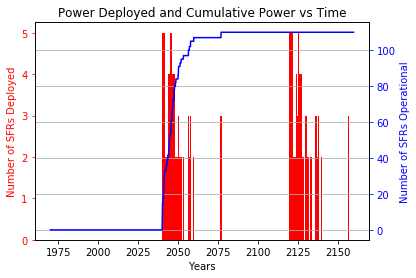
\includegraphics[scale=0.7]{./images/french-transition/sfr_deploy.png}
	\end{center}
	\caption{Deployment of French \glspl{SFR} and total installed capacity}
	\label{fig:dep}
\end{figure}
\FloatBarrier


\Cref{fig:sfr_num} and \cref{fig:dep} display
the French transition to \glspl{SFR} over time.
The steep transition from 2040 to 2060 reflects the scheduled
decommissioning of reactors built in the 1975-2000
era of aggressive nuclear growth in France.


\subsection{Material Definitions}
Depletion calculations of the nuclear fuel are recipe-based, such that a fresh 
and used fuel recipe is used for each reactor type.
For the compositions of the fuel, a reference depletion calculation
from ORIGEN is used (see \cref{tab:comp}). The recipe has also been used for
\cite{wilson_adoption_2009}.


\subsection{Scenario Descriptions}
The simulation follows the model fuel cycle, illustrated in \cref{diag:fc},
where a `source' provides natural uranium, which is enriched by an 'enrichment'
facility to produce \gls{UOX}, while disposing enrichment waste (tails)
to the 'sink' facility. The enriched \gls{UOX} fuels
the \gls{LWR}s and \gls{UOX} waste is produced. The used fuel
is sent to a pool to cool for 3 years \cite{carre_overview_2009}.
The cooled fuel is then reprocessed to separate plutonium and uranium,
or sent to a repository.
The plutonium mixed with depleted uranium (tails) makes \gls{MOX}.
The reprocessed uranium is unused and stockpiled. Uranium is reprocessed
in order to separate the raffinate (Minor actinides and fission products)
from 'usable' material. Though not utilized in this paper, reprocessed
uranium may substitute depleted uranium for \gls{MOX} production. In this
paper, there was sufficient depleted uranium inventory that using reprocessed
uranium was not considered. However, further in the future where the depleted
uranium inventory drains, reprocessed uranium (or, natural uranium) will need to be utilized. 


% Define block styles
\tikzstyle{decision} = [diamond, draw, fill=blue!20, 
text width=4.5em, text badly centered, node distance=3cm, inner sep=0pt]
\tikzstyle{block} = [rectangle, draw, fill=blue!20, 
text width=5em, text centered, rounded corners, minimum height=4em]
\tikzstyle{line} = [draw, -latex']
\tikzstyle{cloud} = [draw, ellipse,fill=red!20, node distance=3cm,
minimum height=2em]


\begin{figure}
        \centering
        \scalebox{0.7}{
                \begin{tikzpicture}[align=center, node distance = 3cm and 3cm, auto]
                % Place nodes
                \node [block] (sr) {Mine (\texttt{SOURCE})};
                \node [cloud, below of=sr] (nu) {Nat U};
                \node [block, below of=nu] (enr) {Enrichment ({\small \texttt{ENRICHMENT}})};
                \node [cloud, below of=enr] (uox) {\gls{UOX}};
                \node [block, below of=uox] (lwr) {\gls{LWR} (\texttt{REACTOR})};
                \node [cloud, right of=lwr] (snf) {\gls{UNF}};
                \node [cloud, right of=uox] (cunf) {Cooled \gls{UNF}};
                \node [block, right of=snf] (pool) {Pool (\texttt{Storage})};
                \node [cloud, left of=lwr] (tl2) {Dep U};
                \node [cloud, right of=enr] (tl) {Dep U};
                \node [block, right of=tl] (sk) {Repository (\texttt{SINK})};
                \node [cloud, below of=pool] (cunf2) {Cooled \gls{UNF}};
                \node [block, below of=snf] (rep) {Reprocessing ({\small \texttt{SEPARATIONS}})};
                \node [cloud, below of=rep] (u) {Sep. U} ;
                \node [cloud, left of=rep] (pu) {Sep. Pu};
                \node [block, left of=pu] (mix) {Fabrication (\texttt{MIXER})};
                \node [cloud, below of=mix] (mox) {\gls{MOX}};
                \node [block, below of=mox] (mxr) {\gls{MOX} Reactors};
                \node [cloud, right of= mxr] (snmox) {Spent \gls{MOX}};
                
                
                \draw[->, thick] (sr) -- (nu);
                \draw[->, thick] (nu) -- (enr);
                \draw[->, thick] (enr) -- (tl);
                \draw[->, thick] (enr) -- (tl2);
                \draw[->, thick] (tl) -- (sk);
                \draw[->, thick] (tl2) -- (mix);
                \draw[->, thick] (enr) -- (uox);
                \draw[->, thick] (uox) -- (lwr);
                \draw[->, thick] (lwr) -- (snf);
                
                \draw[->, thick] (lwr) -- (snf);
                \draw[->, thick] (snf) -- (pool);
                \draw[->, thick] (pool) -- (cunf);
                \draw[->, thick] (pool) -- (cunf2);
                \draw[->, thick] (cunf) -- (sk);
                \draw[->, thick] (cunf2) -- (rep);
                
                \draw[->, thick] (rep) -- (u);
                \draw[->, thick] (rep) -- (pu);
                \draw[->, thick] (pu) -- (mix);
                \draw[->, thick] (mix) -- (mox);
                \draw[->, thick] (mox) -- (mxr);
                \draw[->, thick] (mxr) -- (snmox);
                \draw[->, thick] (snmox) -- (rep);
                
                \end{tikzpicture}
        
                }
                \caption{Model Fuel Cycle with \gls{MOX} Reprocessing}
                \label{diag:fc}
\end{figure}


The second scenario separates plutonium from the \gls{UNF}
inventory from the previous simulation. The separated
plutonium mixed with the depleted uranium inventory from the previous simulation
creates \gls{MOX}, which fuels the \gls{SFR}s. 

\section{Scenario Specifications}
%% EARLY???
This paper shows results from two separate simulations.
The first simulation is a historical operation of \gls{EU} reactors, with a
realistic reprocessing and \gls{MOX} fabrication capacity, 
modeled after the French La Hague and MELOX site \cite{schneider_spent_2008, hugelmann_melox_1999}.
The second simulation is an ideal French Transition scenario to \gls{SFR},
where an ASTRID-type \gls{SFR} replaces the decommissioned
capacity of \glspl{LWR} in France. The specifications of the simulations
are listed in tables \ref{tab:sim_eu} and \ref{tab:sim_france}.

\begin{table}[h]
	\centering
	\begin{tabularx}{\textwidth}{bb}
		\hline
		Parameter & Value \\
		\hline
		Simulation Time & 1970-2050 \\ 
		Reprocessing Capacity & 91.6 MTHM of \gls{UNF} per month \cite{schneider_spent_2008} \\
		Reprocessing Efficiency & 99.8\% \\
		Reprocessing Streams & Plutonium and Uranium \\
		\gls{MOX} Fabrication & \small{9\% Reprocessed Pu + 91\% Depleted U} \\
		\gls{MOX} Fabrication Throughput & 16.25 MTHM of \gls{MOX} per month  \cite{hugelmann_melox_1999} \\
		\gls{MOX} Fuel Reprocessing Stage &  Used \gls{MOX} gets reprocessed infinitely. \\  
		Reprocessed Uranium Usage &  None. Stockpile reprocessed U \\
		\hline
	\end{tabularx}
	\caption {Specification for Historical Operation of \gls{EU} Case}
	\label{tab:sim_eu}
\end{table}

\begin{table}[h]
	\centering
	\begin{tabularx}{\textwidth}{bb}
		\hline
		Parameter & Value \\
		\hline
		Simulation Time & 1970-2160 \\
		\gls{SFR} Available Year & 2040 \\
		Reprocessing Capacity & $\infty$ \\
		Reprocessing and Fabrication Begins & 2020 \\
		Separation Efficiency & 99.8 \% \\
		Reprocessing Streams & plutonium and uranium \\
		\small{Used \gls{UOX} and Depleted U Inventory} & 141,659 MTHM {\small (From first simulation)} \\
		\small{Additional Used \gls{UOX} or Depleted U} & None  \\
		\gls{MOX} Fabrication &  \small{11\% Reprocessed Pu + 89\% Depleted U}  \\
		\gls{MOX} Fabrication Throughput & infinite \\
		\gls{MOX} Fuel Reprocessing Stage &  Used \gls{MOX} gets reprocessed infinitely. \\
		Reprocessed Uranium Usage &  None. Stockpile reprocessed U. \\
		\hline
	\end{tabularx}
	\caption {Specification for French Transition to \gls{SFR} case }
	\label{tab:sim_france}
\end{table}


\section{Reactor Specifications}
Three major reactors are used in the simulation, \gls{PWR}, gls{BWR}, and ASTRID - type reactors.

For \glspl{PWR}, a linear core size model was assumed to capture
varying reactor capacity. For example, a 
1,000 MWe PWR has 193 \gls{UOX} assemblies, each
weighing 523.4 kg.
After each 18 month cycle, one-third of the 
core (64 assemblies) discharge. Refueling
is assumed to take 2 months to complete, during which the reactor
is shut down. This value is acquired by averaging the 
historical refueling outage. The specifications are defined in \cref{tab:pwr}.

For \glspl{BWR}, a linear core size model was assumed to capture
varying reactor capacity as well. It assumed a assembly size of
180 kg, with 1000 MWe BWR plant having 764 assemblies, adjusted
linearly by capacity. The refueling cycle is identical to that
of a \gls{PWR}. The specifications are defined in \cref{tab:bwr}.

For the \gls{SFR}, a model design is adopted from
Marsault-Marie-Sophie et al. \cite{marsaultmarie-sophie_pre-conceptual_2012}.
The specifications are defined in \cref{tab:sfr}.

\begin{table}[h]
	\centering
	\begin{tabularx}{\textwidth}{bb}
		\hline
		Parameter & Value \\
		\hline
		PWR Cycle Time & 18 months \\ 
		PWR Refueling Outage & 2 months \\
		Fuel Mass per Assembly & 523.4 kg \\
		Burnup & 51 GWd/tons \\
		Num. of Aseem. per Core & 193 for 1,000 MWe, linearly adjusted\\
		Num. of Assem. per Batch & 1/3 of the core \\
		Fuel & \small{French \glspl{PWR} prefer \gls{MOX} but also accept \gls{UOX}}\\
		\hline
	\end{tabularx}
	\caption {\gls{PWR} Specifications}
	\label{tab:pwr}
	\end{table}
	
\begin{table}[h]
	\centering
	\begin{tabularx}{\textwidth}{bb}
		\hline
		Parameter & Value \\
		\hline
		BWR Cycle Time & 18 months \\ 
		PWR Refueling Outage & 2 months \\
		Fuel Mass per Assembly & 180 kg \\
		Burnup & 51 GWd/tons \\
		Num. of Aseem. per Core & 764 for 1,000 MWe, linearly adjusted\\
		Num. of Assem. per Batch & 1/3 of the core \\
		\hline
	\end{tabularx}
	\caption {\gls{BWR} Specifications}
	\label{tab:bwr}
\end{table}
	
\begin{table}[h]
	\centering
	\begin{tabularx}{\textwidth}{bb}
		\hline
		Parameter & Value \\
		\hline
		SFR Cycle Time & 12 months \\ 
		SFR Refueling Outage & 2 months \\
		Fuel Mass per Batch & 11,136 kg \\
		Batch per Core & 4 \\
		Power Output & 600 MWe \\
		lifetime & 80 years \\
		Fuel & {\small \gls{MOX} (89\% Tailings, 11\% Separated Pu)}\\
		\hline
	\end{tabularx}
	\caption {\gls{SFR} ASTRID Specifications \cite{marsaultmarie-sophie_pre-conceptual_2012}}
	\label{tab:sfr}
\end{table}
\FloatBarrier


\section{Future Nuclear Projections}

The future of nuclear energy in \gls{EU} nations is organized
in the table by the World Nuclear Association \cite{world_nuclear_association_nuclear_2017}.
It is assumed in the simulations that all the planned constructions 
are completed on their expected date without delay
or failure. Also, the newly constructed nuclear power plants are assumed to have a lifetime of 60 years.

\Cref{tab:eu_deployment} lists the reactors that are currently  planned or under construction.

 
\begin{table}[h]
	\centering
	\caption {Power Reactors under construction and planned \cite{world_nuclear_association_nuclear_2017}}
	\label{tab:eu_deployment}
	\begin{tabular}{lllcr}
		\hline
		Start & Nation & Reactor & Type & Capacity\\
                $[yr]$ & & & & $[MW_e]$\\
		\hline
		2018 & Slovakia  & Mochovce 3 & PWR & 440\\
		2018 & Slovakia & Mochovce 4 & PWR & 440 \\
		2018 & France & Flamanville 3 & PWR & 1600 \\
		2018 & Finland & Olkilouto 3 & PWR & 1720 \\		
		2019 & Romania & Cernavoda 3 & PHWR & 720 \\
		2020 & Romania & Cernavoda 4 & PHWR & 720 \\
		2024 & Finland & Hanhikivi & VVER1200 & 1200 \\
		2024 & Hungary & Paks 5 & VVER1200 & 1200 \\
		2025 & Hungary & Paks 6 & VVER1200 & 1200 \\
		2025 & Bulgaria & Kozloduy 7 & AP1000? & 950 \\
		2026 & UK & Hinkley Point C1 & EPR & 1670 \\
		2027 & UK & Hinkley Point C2 & EPR & 1670 \\
		2029 & Poland & Choczewo & N/A & 3000 \\
		2035 & Poland & N/A & N/A & 3000 \\
		2035 & Czech Rep & Dukovany 5 & N/A & 1200 \\
		2035 & Czech Rep & Temelin 3 & AP1000 & 1200 \\
		2040 & Czech Rep & Temelin 4 & AP1000 & 1200 \\
		\hline
	\end{tabular}
\end{table}
\FloatBarrier

For each \gls{EU} nation, the growth trajectory is categorized from
``Aggressive Growth'' to ``Aggressive Shutdown''. Aggressive growth is
characterized by a rigorous expansion of nuclear power while 
Aggressive Shutdown is characterized as a transition to rapidly
de-nuclearize the nation's electric grid. A nation's growth trajectory is
categorized into five degrees depending on x, 
given by $\frac{Nuclear\ capacity\ in\ 2040}{Nuclear\ capacity\ in\ 2017}$.

\begin{itemize}
	\item Aggressive Growth ($x \geq 2$)
	\item Modest Growth ($1.2 \leq x < 2$)
	\item Maintenance ($0.8 \leq x < 1.2$)
	\item Modest Reduction ($0.5 \leq x< 0.8$)
	\item Aggressive Reduction ($x \leq 0.5$)
\end{itemize}

The growth trajectory and specific plan of each nation in the \gls{EU} 
is listed in Table \ref{tab:eu_growth}.

\begin{table}[h]
	\centering
		\begin{tabularx}{\textwidth}{smb}
			\hline 
			
			Nation & Growth Trajectory & Specific Plan \\
			\hline \hline
			UK & Aggressive Growth & 13 units (17,900 MWe) by 2030.\\
			\hline
			Poland & Aggressive Growth & Additional 6,000 MWe by 2035.\\
			\hline
			Hungary & Aggressive Growth & Additional 2,400 MWe (VVER-1200) by 2025. \\ 
			\hline
			Finland & Modest Growth & Additional EPR in 2018, VVER in 2024.\\
			\hline
			Bulgaria & Modest Growth & Additional AP1000 (1,000 MWe) construction in 2035. \\
			\hline
			Romania & Modest Growth & Additional 1,440 MWe by 2020. \\
			\hline
			Czech Rep. & Modest Growth & Additional 2,400 MWe (AP1000s) by 2035.\\
			\hline
			France & Maintenance & Shutdown nuclear plants if they reach end of lifetime. No new construction.\\
			\hline
			Spain & Modest Reduction & No plans to expand or early shutdown. \\
			\hline
			Italy & Modest Reduction & No plans to expand or early shutdown. \\
			\hline
			Belgium & Aggressive Reduction & All shut down 2025.\\
			\hline
			Sweden & Aggressive Reduction & All shut down 2050.\\
			\hline
			Germany & Aggressive Reduction & All shut down by 2022.\\
			\hline
			
		\end{tabularx}

	\caption {Future Nuclear Programs of \gls{EU} Nations \cite{world_nuclear_association_nuclear_2017}}
  \label{tab:eu_growth}
\end{table}
\FloatBarrier

\section{Results}

\subsection{Historical Operation of \gls{EU} Reactors}

\Cref{tab:sim_result} lists the important metrics
obtained from the first simulation. The following
values are the \gls{EU} inventory and history at year 2050,
and will be reprocessed in the second simulation.

\begin{table}[h]
	\centering
%	\scalebox{0.86}{
		\begin{tabular}{|c|c|c|c|}
			\hline
			Category & Unit & Value & Specifics\\ \hline
			Total UOX Usage & MTHM & 181,471 &  \\ \hline
			Total MOX Usage & MTHM & 6,302 & \\ \hline
			Total Used UOX Stored & MTHM & 141,659 & \gls{UNF} that is not reprocessed\\ \hline
			Total Used  MOX Stored & MTHM & 3,611 & \gls{UNF} that is not reprocessed \\ \hline
			Total Tailings & MTHM & 1,081,826 & \\ \hline
			Total Natural U Used & MTHM & 1,269,897 & \\ \hline
		\end{tabular}
		\caption{Simulation Results for Historical Nuclear Operation of \gls{EU} Nations}
		\label{tab:sim_result}
\end {table}
\FloatBarrier


Figures \ref{fig:eu_tail} and \ref{fig:eu_snf} show the 
timeseries of mass of tailings and used fuel accumulation in \gls{EU}.
Figure \ref{fig:eu_fuel} shows the amount of fuel used in \gls{EU}.


\begin{figure}[htbp!]
	\begin{center}
		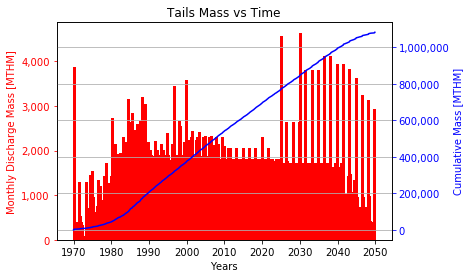
\includegraphics[scale=0.7]{./images/eu_future/tails.png}
	\end{center}
	\caption{Timeseries of Tails Mass in the \gls{EU}.}
	\label{fig:eu_tail}
\end{figure}

\begin{figure}[htbp!]
	\begin{center}
		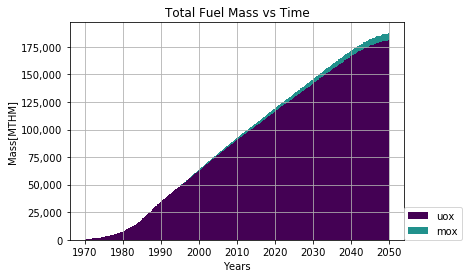
\includegraphics[scale=0.7]{./images/eu_future/total_fuel.png}
	\end{center}
	\caption{Timeseries of Total Fuel Usage in \gls{EU}.}
	\label{fig:eu_fuel}
\end{figure}


\begin{figure}[htbp!]
	\begin{center}
			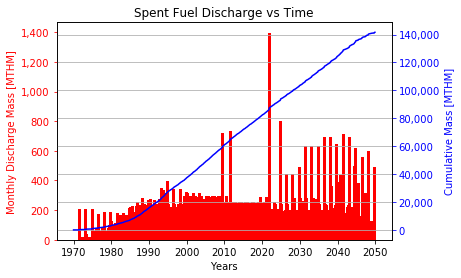
\includegraphics[scale=0.7]{./images/eu_future/snf_discharge.png}
	\end{center}
	\caption{Timeseries of Used Nuclear Fuel in \gls{EU}.}
	\label{fig:eu_snf}
\end{figure}
\FloatBarrier


\begin{table}[h]
	\centering
	\begin{tabular}{|c|c|c|}
		\hline
		Isotope & Mass Fraction in Used Fuel [\%] & Quantity [t] \\ \hline
		Total & 0.9358 & 1,325 \\ \hline
		Pu238 & 0.0111 & 15.72 \\ \hline
		Pu239 & 0.518 & 733.79 \\ \hline
		Pu240 & 0.232 & 328.64 \\ \hline
		Pu241 & 0.126 & 178.49 \\ \hline
		Pu242 & 0.0487 & 68.98 \\ \hline
	\end{tabular}
	\caption{Plutonium From Used Fuel}
	\label{tab:pu}
\end{table}


\Cref{tab:pu} lists the isotope, mass fraction,
and quantity of plutonium that can be obtained from the 2050 \gls{UNF} inventory.


\subsection{French \gls{SFR} Transition Scenario}

Reprocessing \gls{UNF} collected from all EU nations can start approximately
270 \glspl{SFR}, which is more than enough for two generations of 66GWe \gls{SFR}
fleet. With the \gls{SFR} breeding ratio of over one, France can transition into
a fully \gls{SFR} fleet without extra construction of \glspl{LWR}. 

From Varaine et al. \cite{marsaultmarie-sophie_pre-conceptual_2012}, a French
ASTRID-type \gls{SFR} of capacity 600 MWe needs $1.225$ tons of
plutonium a year, with an initial plutonium loading of $4.9$ tons. 
Thus, the number of \glspl{SFR} that can be loaded with the reprocessed
plutonium from \gls{UNF} can be estimated to $\frac{Pu \ from \ legacy \ \gls{UNF}}{4.9} \approx 270$ \glspl{SFR},
assuming infinite reprocessing and fabrication capacity as well as
abundant depleted uranium supply. 

Also, assuming that \gls{MOX} can be recycled indefinitely,
used \gls{MOX} from an ASTRID reactor contains enough plutonium to produce a \gls{MOX} fuel with
the same mass, if mixed with depleted uranium. For example,
used \gls{MOX} from an ASTRID reactor is assumed to be 12.6\% plutonium
in this simulation (see \cref{tab:comp}), whereas a fresh \gls{MOX} is 11\% plutonium.
Separating plutonium from used \gls{MOX} from
an ASTRID reactor can create \gls{MOX} of the mass of used \gls{MOX}.
The plutonium breeding ratio in this simulation is thus assumed to be
$\approx 1.145$.

\Cref{fig:fuel} shows \gls{MOX} loaded in the \glspl{SFR} per month.
The spikes are due to initial fuel demand for new deployment of \glspl{SFR}.
The initial loading of new \glspl{SFR} are done with the \gls{MOX} created
from legacy \gls{UNF}. Once there are enough amounts of extra plutonium creation
by deployed \glspl{SFR}, the legacy \gls{UNF} is no longer used. 

\begin{figure}[htbp!]
	\begin{center}
		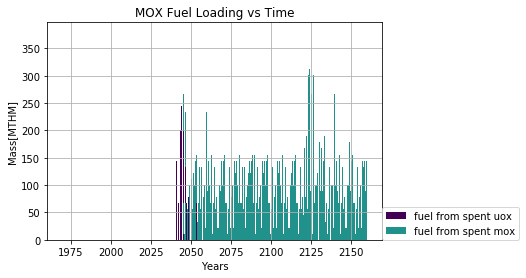
\includegraphics[scale=0.7]{./images/french-transition/where_fuel.png}
	\end{center}
	\caption{Timeseries of fuel loaded into \glspl{SFR}}
	\label{fig:fuel}
\end{figure}

\Cref{fig:reprocess_waste} shows the amount of reprocessing waste
(minor actinides, fission products) over time. The spikes in the 
waste discharge is due to large influx of spent fuel from
decommissioned \glspl{SFR}.\Cref{fig:pu_no_cum} shows the separated plutonium discharge
per month from the reprocessing plant. The plutonium outflux
does not precisely follow the fuel demand because \Cyclus agents have
material buffers that store commodity fuel for later usage. 
\Cref{tab:sfr_sim_result} lists metrics obtained from the second simulation.

\begin{figure}[htbp!]
	\begin{center}
		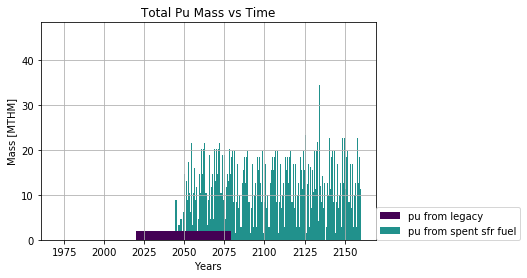
\includegraphics[scale=0.7]{./images/french-transition/pu.png}
	\end{center}
	\caption{Separated plutonium discharge from Reprocessing Plant}
	\label{fig:pu_no_cum}
\end{figure}


\begin{figure}[htbp!]
	\begin{center}
		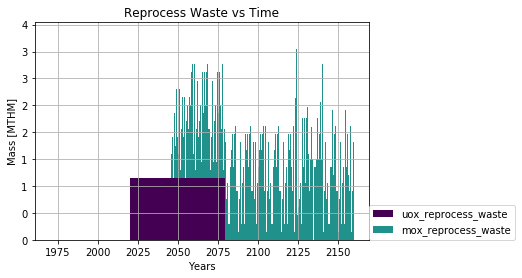
\includegraphics[scale=0.7]{./images/french-transition/reprocess_waste.png}
	\end{center}
	\caption{Reprocessing waste discharge from Reprocessing Plant}
	\label{fig:reprocess_waste}
\end{figure}


\begin{table}[h]
	\centering
	\scalebox{0.86}{
		\begin{tabular}{|c|c|c|}
			\hline
			Category & Unit & Value  \\ \hline
			Total MOX used & MTHM & 127,640  \\ \hline
			Total \glspl{SFR} Deployed & & 220 \\ \hline
			Total Plutonium Reprocessed & MTHM & 16,352 \\ \hline
			Total MOX from UOX Waste & MTHM & 6,570  \\ \hline
			Total MOX from MOX Waste & MTHM  & 121,070 \\ \hline
			Total Tails used & MTHM & 116,153 \\ \hline
			Total legacy UNF reprocessed & MTHM & 77,082 \\ \hline
			Total Reprocessed Uranium Stockpile & MTHM & 184,172 \\ \hline
			Total Reprocess Waste & MTHM & 16,352 \\ \hline
		\end{tabular}}
		\caption {\gls{SFR} Simulation Results}
		\label{tab:sfr_sim_result}
\end {table}



\section{Discussion}
This work demonstrated that, with reprocessing capacity of 250 MTHM per month,
and a fabrication capacity of 300 MTHM per month,
France, by receiving \gls{UNF} from other \gls{EU} nations,
 can transition into, for unchanging nuclear electricity demand,
a fully \gls{SFR} fleet
with installed capacity of 66,000 MWe by 2076.
\gls{MOX} from reprocessed \gls{UNF} meets the initial fuel demand,
which later on is supplied by \gls{MOX} created from recycled \gls{MOX}.

Since most \gls{EU} nations do not have an operating \gls{UNF}
repository or a management plan, they have a strong incentive
to send all their \gls{UNF} to France. The nations
with aggressive nuclear reduction will be able phase out nuclear
without constructing a High Level Waste repository. France has an
incentive to take this fuel, since reuse of used fuel from
other nations will allow France to meet their MOX demand
without new construction of \glspl{LWR}.

Though complex political and economic factors are not
addressed, and various assumptions present for this scenario,
this option may hold value for the \gls{EU} as a nuclear community,
and for France to advance into a closed fuel cycle.


\bibliographystyle{abbrv}
\bibliography{./bibliography.bib}

\input{appendix.tex}



\end{document}
\grid
